%%%%%%%%%%%%%%%%%%%%%%%%%%%%%%%%%%%%%%%%%%%%%%%%%%%
% DECLARATION DE LA CLASSE DU DOCUMENT
%%%%%%%%%%%%%%%%%%%%%%%%%%%%%%%%%%%%%%%%%%%%%%%%%%%
%% Les fichier dans le répertoire couverture contiennent les informations qui vont s'afficher sur la page de couverture. 
%%Option du type de rapport : memoireMaitrise; projetTutore; projetSemestre; memoireLicence; projet; miniProjet

\documentclass[
    a4paper,        %%% Format du papier : a4paper, letter, ...
    oneside,        %%% recto ou recto-verso : oneside, twoside.
    12pt,           %%% Taille par défaut des polices
    memoireMaitrise,%%% Type de rapport à produire : memoireMaitrise, projetTutore, memoireLicence, ....
    francais,       %%% Langue du document
    creativecommons,%%% Affichage de la licence d'utilisation du document : reserved, creativecommons
    hyperref,       %%% Utilisation de lien hypertexte
    withAlgo2e      %%% Utilisation de l'algorithme dans le document
]{memoESPA}

\makenomenclature
\makeindex

% DECLARATION D'UNE LISTE DE RÉFÉRENCES SUPPLÉMENTAIRE
\newcites{refs}{WEBOGRAPHIE}
%%% Inclusion des fichiers nécessaires pour les pages de titre et de garde
%% Informations sur le rapport
% PAGE TITRE
%%% Veuillez changer le contenu de ce fichier pour le faire correspondre au votre 
\title{Titre du mémoire ou Projet }     %% Le titre du projet ou mémoire
\author{NOM DE FAMILLE Prénoms }        %% Le nom et prénoms du candidat
\authorcopyright{Nom Prénoms }          %% Le nom et prénoms du candidat
\datesoutenance{\today}                 %% Date prévue de la soutenance ex. \datesoutenance{25 Janvier 2027}
\datedepot{\today}                      %% Date de dépôt de la version finale du rapport ex. \datedepot{\18 Janvier 2027}
\ecole{ÉCOLE SUPÉRIEURE POLYTECHNIQUE D’ANTSIRANANA} %% Nom de l'établissement
\mention{Sciences et Technologies de l'Information et de la Communication} %% Mention d'affiliation
\parcours{Électronique et Informatique Industrielle} %% Parcours dans la mention
\anneeU{2024 - 2025}                    %% Année universitaire en cours
\promo{Nom de la promo}                    %% Nom de la promotion si c'est un mémoire
%% Liste des encadreurs
%%% Veuillez changer le contenu de ce fichier pour le faire correspondre au votre 
%%% Remplacer par les noms et prénoms des encadreurs par des noms réels
%%% Vous pouvez ajouter jusqu'à 6 encadreurs, seul le premier est obligatoire
%%% Commentez le reste pour ne pas les afficher sur la page de couverture
%%% Si un encadreur fait partie des membres du jury, ajoutez le mot "jury" à la dernière section de la variable
%%% Si l'encadreur n'est pas membre du jury, laissez vide la dernière section
\encadreurA{Pr.}{Nom et Prénom du 1 er encadreur}{Encadreur}{jury}
\encadreurB{Dr.}{Nom et Prénom du 2 ème encadreur}{Encadreur}{jury}
\encadreurC{Mme.}{Nom et Prénom du 3 ème encadreur}{Encadreur}{}
%\encadreurD{Mr.}{Nom et Prénom du 4 ème encadreur}{Encadreur}{}
%\encadreurE{Mme.}{Nom et Prénom du 5 ème encadreur}{Encadreur}{}
%\encadreurF{Mr.}{Nom et Prénom du 6 ème encadreur}{Encadreur}{}
%% Liste des jurys 
%%% Veuillez changer le contenu de ce fichier pour le faire correspondre au votre 
%%% Remplacer par les noms et prénoms des membres du jury 
%%% Vous pouvez ajouter jusqu'à 4 examinateurs, seul le président du jury est obligatoire
%%% Commentez le reste pour ne pas les afficher sur la page de couverture

\president{Pr.}{Nom et Prénom du Président du jury}{Président}
%\examinateurA{Pr.}{Nom et Prénom du 1 ier examinateur}{Examinateur}
\examinateurB{Dr.}{Nom et Prénom du 2 ème examinateur}{Examinateur}
\examinateurC{Mme.}{Nom et Prénom du 3 ème examinateur}{Examinatrice}
%\examinateurD{Mr.}{Nom et Prénom du 4 ème examinateur}{Examinateur}

%% Configuration des commandes pour un algorithme
\SetKwProg{Fn}{Function}{}{}
\SetKwProg{Pr}{Procedure}{}{}
\SetKwInOut{Variable}{var}
\SetKwInput{KwData}{Algorithme}
\SetKw{End}{end}
\SetKw{Kw}{}
\makeindex
%%%%%%%%%%%%%%%%%%%%%%%%%%%%%%%%%%%%%%%%%%%%%%%%%%%
% INTITULÉ DU DIPLOME
%%%%%%%%%%%%%%%%%%%%%%%%%%%%%%%%%%%%%%%%%%%%%%%%%%%
\listfiles
%%%%%%%%%%%%%%%%%%%%%%%%%%%%%%%%%%%%%%%%%%%%%%%%%%%
% DÉBUT DU DOCUMENT
%%%%%%%%%%%%%%%%%%%%%%%%%%%%%%%%%%%%%%%%%%%%%%%%%%%
\begin{document}

\pagenumbering{Roman}
%%- Affichage de la page titre -%%
\maketitle

%%- Affichage de la présentaiton du jury -%%
\presentjury

%%%- Avant propos -%%
%% avantpropos
\begin{avantpropos}

\lipsum[1] % Texte de remplissage pour donner un exemple de la mise en page

\end{avantpropos}

%%- Remerciements -%%
%%- Remerciements -%%
\begin{remerciements}

\lipsum[3-4] % Texte de remplissage pour donner un exemple de la mise en page

\end{remerciements}

%%- Sommaire  et abstract-%%
%%- Sommaire -%%
\begin{sommaire}{mot-clé1, mot-clé2, ...}

\lipsum[1]\cite{InProceedingsComExample} % Texte de remplissage pour donner un exemple de la mise en page

\end{sommaire}


%%- Abstract -%%
\begin{abstract}{Titre en anglais}{keyword1, keyword2, ...}

\lipsum[1] \citep{online}% Texte de remplissage pour donner un exemple de la mise en page

\end{abstract}

%%- Affichage de la table des matières -%%
\tableofcontents

%%- Affichage de la liste des tableaux -%%
\listoftables

%%- Affichage de la liste des Figures -%%
\listoffigures

%%- Déclaration et affichage de la liste des abbréviations -%%
%%- Déclaration et affichage de la liste des abbréviations -%%
\begin{listofabbr}[3cm]
\item [ESPA] École Supérieure Polytechnique
\item [STIC] Sciences et Technologies de l’Information et de la Communication
\item [EII] Électronique et Informatique Industrielle
\item [TR] Télécommunication et Réseaux
\item [Z...] .......
\end{listofabbr}



%%- Déclaration et affichage de la liste des symboles -%%
%%- Déclaration et affichage de la liste des symboles -%%
\begin{listofsymbols}[3cm]
\item [a] Première lettre de l'alphabet
\item [A] Ampère : l'unité de mesure du courant 
\item [$\pi$] Le nombre pi = 3.141
\item [...] ...
\end{listofsymbols}

\cleardoublepage

\pagenumbering{arabic}

%% Marginpar à gauche du document
\reversemarginpar

%%%%%%%%%%%%%%%%%%%%%%%%%%%%%%%%%%%%%%%%%%%%%%%%%%%
% EXEMPLE DE CORPS DE MÉMOIRE
%%%%%%%%%%%%%%%%%%%%%%%%%%%%%%%%%%%%%%%%%%%%%%%%%%%

%% Introduction
%% introduction
\begin{introduction}

\lipsum[1] % Texte de remplissage pour donner un exemple de la mise en page

\lipsum[2-3]

\end{introduction}


%%- Premier chapitre de démonstration -%%
%%- Premier chapitre de démonstration -%%
\chapter{Test de long titre de Chapitre, avec retour à la ligne. Lorem ipsum dolor sit amet, consectetur adipiscing elit. Pellentesque justo justo, porta sagittis feugiat eget, ornare rhoncus ligula. Nunc non odio sed lacus rutrum rhoncus.}


\section{Tests de mise en page}

Dans cette section, différents environnements de mise en page sont présentés.

\subsection{Figure simple}

    Insertion d'une figure dont le numéro est Fig. \ref{figureSimple}
    \begin{figure}
    	\centering % Les figures doivent être centrées
    	
\includegraphics[width=0.5\textwidth]{figures/logoUNA.jpg}
            \caption{Insertion d'une figure simple}\label{figureSimple}
    \end{figure}

\lipsum[1]
\subsection{Figures avec légende longue}
    Exemple de déclaration de figure
    \begin{figure}
        \centering % Les figures doivent être centrées
        
\includegraphics[width=0.5\textwidth]{figures/logoESPA.png} % 
        \\ \parbox{0.75\textwidth}{\caption{Test de longue légende, avec utilisation de framebox et parbox pour restreindre la largeur de la légende.}\label{logoESPA}} % Utilisation d'une parbox pour restreindre la largeur de la légende.
    \end{figure}
\lipsum[2]
\subsection{Insertion de plusieurs figures}

Ci-après est un exemple d'insertion de deux figures cote à cote.

        \begin{figure*}[!h]
		\begin{center}
			\subfloat[Recherche de la meilleure réponse]{
				\label{org-brm001}
					\hspace{0.5cm}
					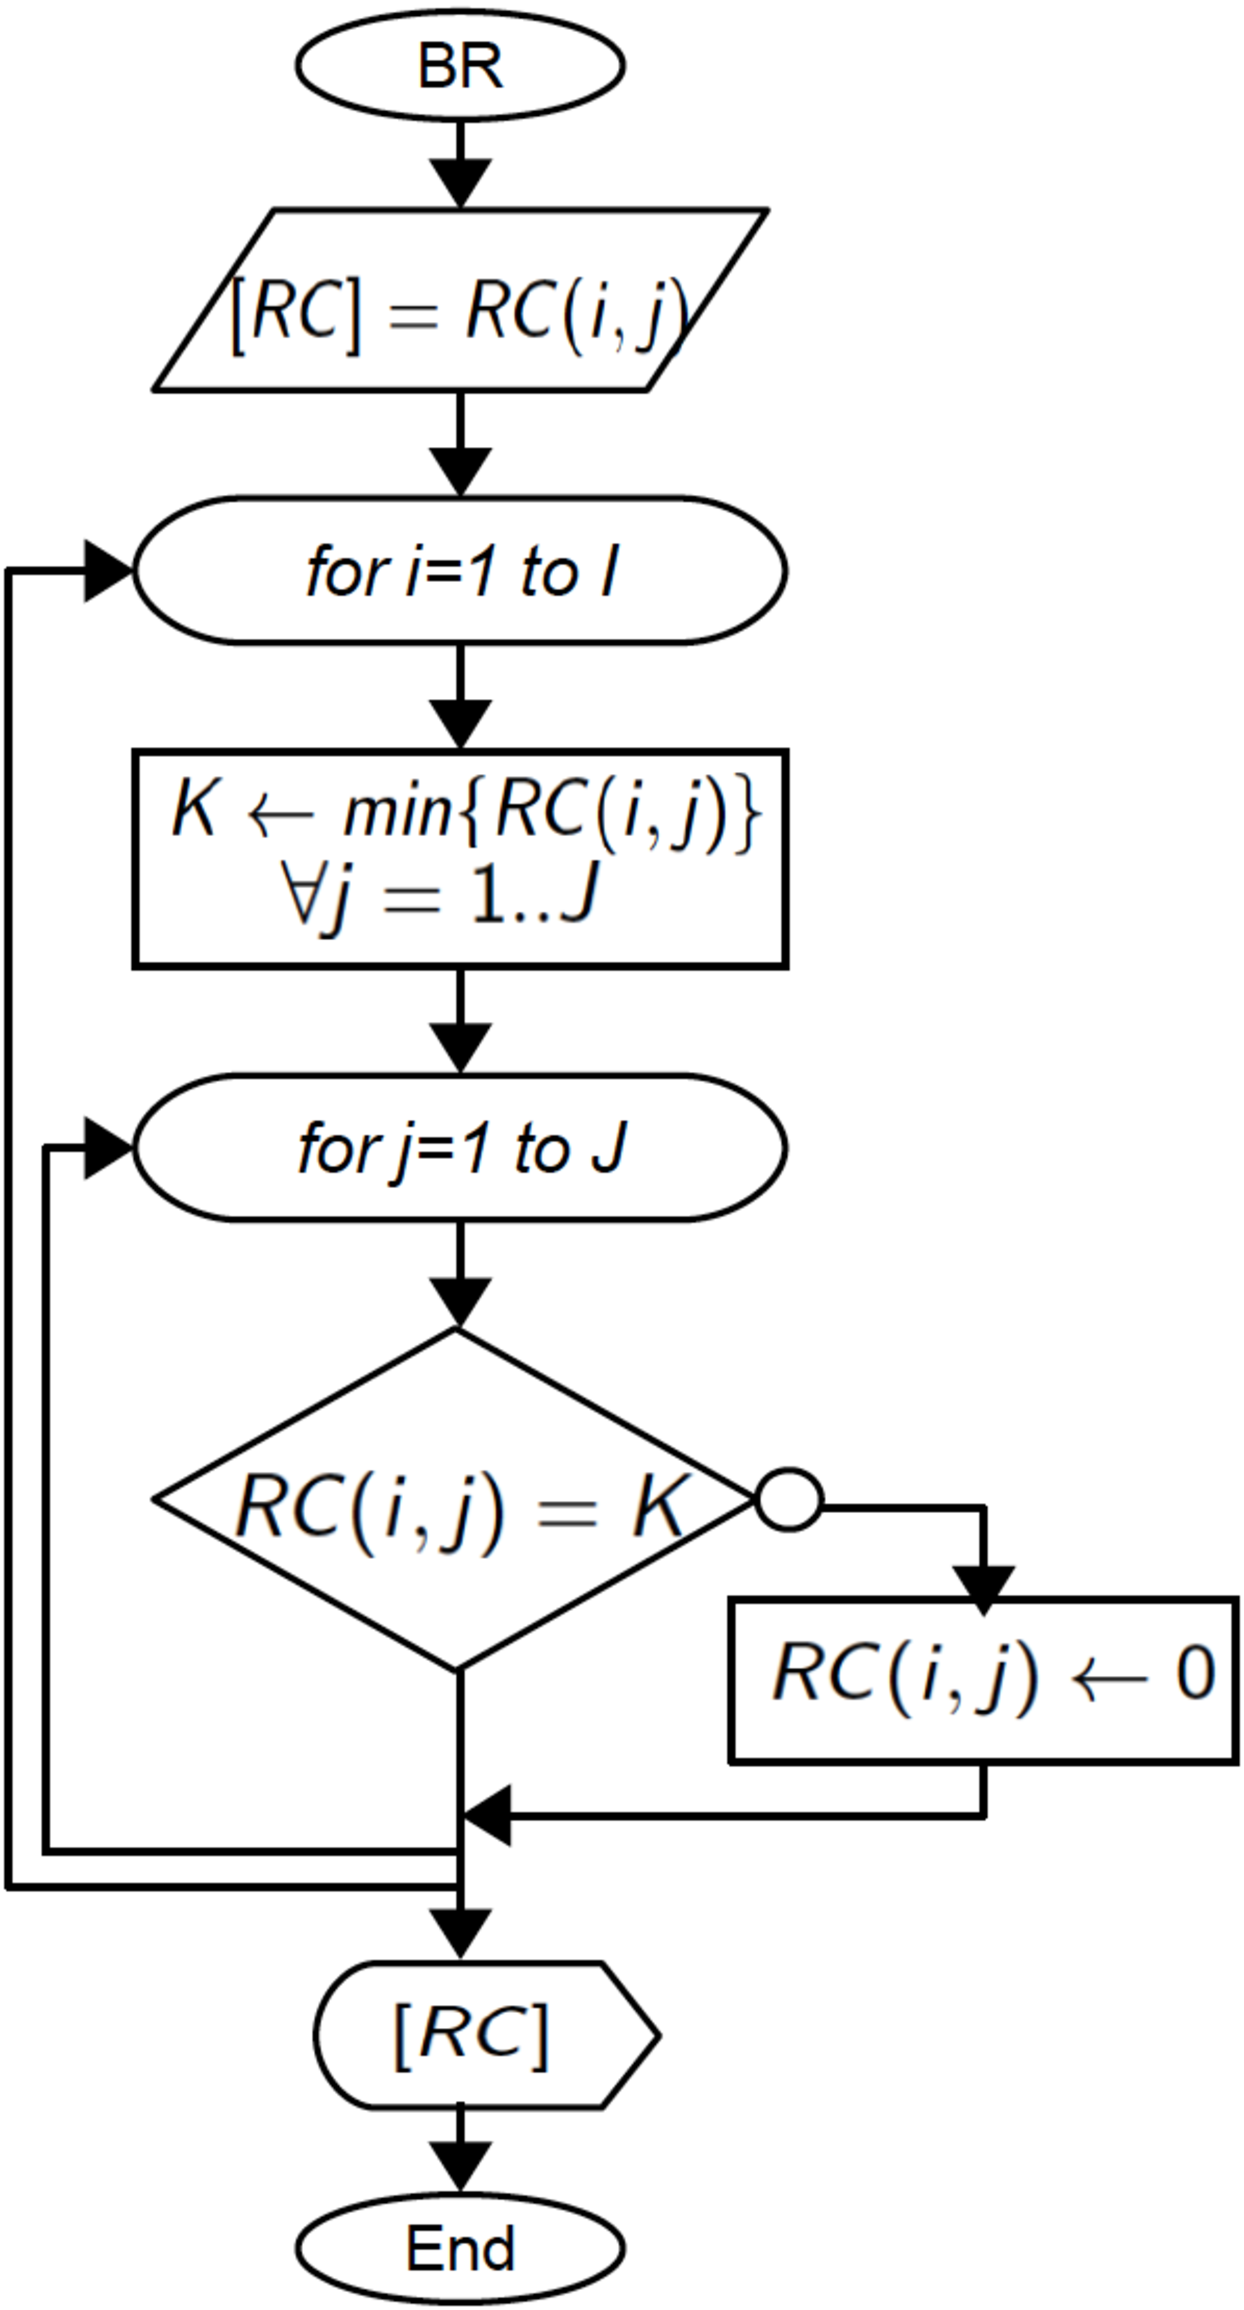
\includegraphics[width=0.41\textwidth]{figures/org-brm001}
					\hspace{0.4cm}
			}\hfill
			\subfloat[Sélection des meilleures réponses]{
				\label{org-brm002}
					\hspace{0.7cm}
					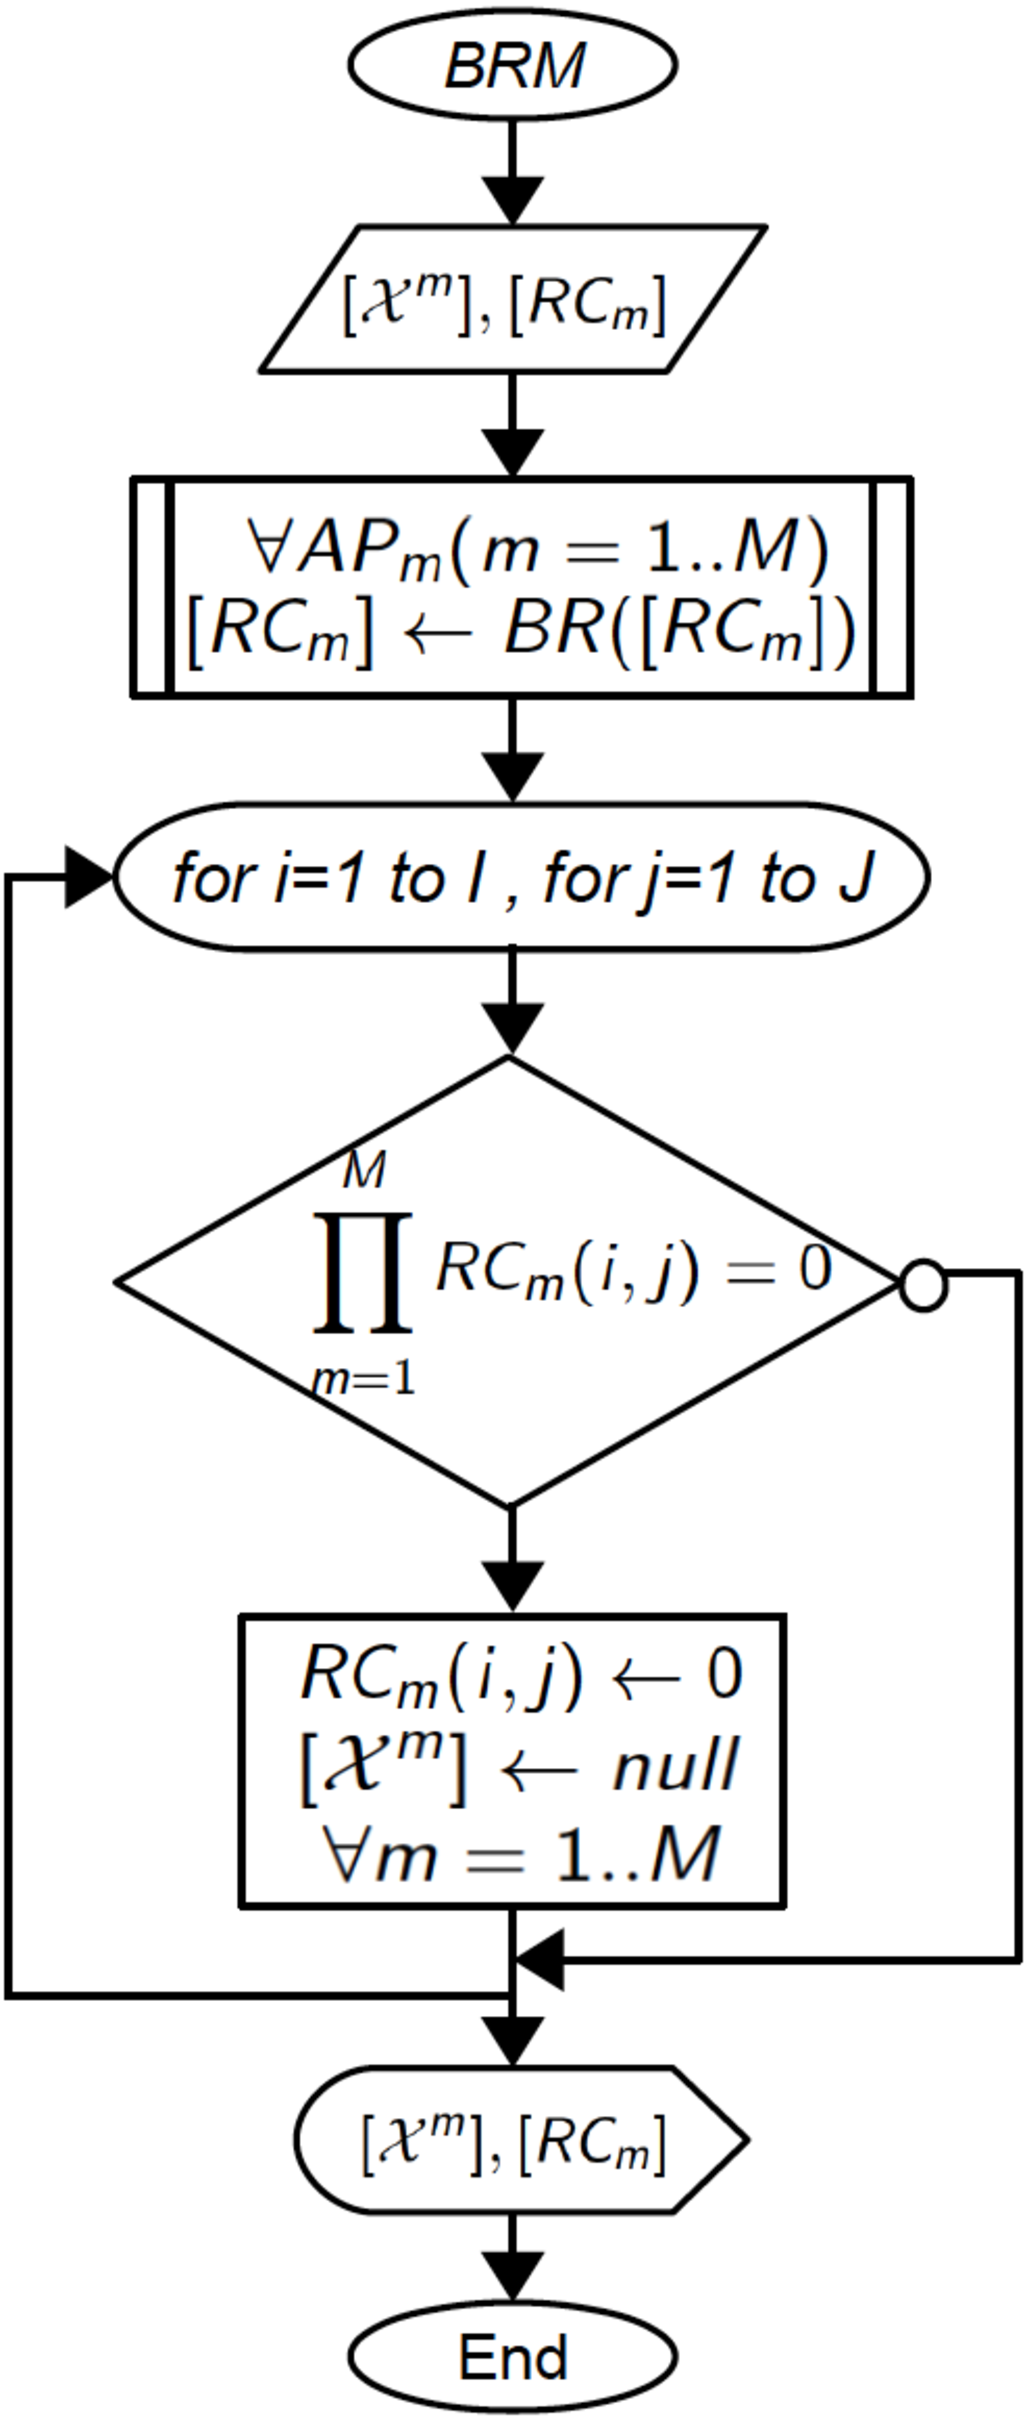
\includegraphics[width=0.322\textwidth]{figures/org-brm002}
					\hspace{0.8cm}
			}\hfill
			\caption{Illustration de l'utilisation de la méthode BRM}
			\label{org-brm}
		\end{center}
	\end{figure*}

La figure \ref{org-brm001} (de la page \pageref{org-brm001}) représente le premier organigramme et la figure \ref{org-brm002} (de la page \pageref{org-brm002}) le deuxième organigramme.

\subsection{Test des listings}

Présentation des principaux listings: les énumations et les listes.

\subsubsection{Énumérations: environement enum}

Test de l'environnement enum:
\begin{enumerate}
 \item test 1
 \item test 2
\end{enumerate}

\subsubsection{Listes: environement itemize}

Test de l'environnement itemize
\begin{itemize}
 \item test 1
 \item test 2
\end{itemize}

\subsection{Test des équations}

Mise en page des équations

\begin{equation}
   \beta = 8 \label{equation1}
\end{equation}

\begin{equation}
   \bm{\gamma} = \alpha \times 3
\end{equation} \label{equation2}

\subsection{Insertion d'une longue équation }

L'équation \ref{equation3} est un exemple d'équation, longue présentée sur plusieurs lignes.
    \begin{multline}
	C_m(SP_{\lambda}) = \Big(\underset{U_m \text{ fois }}{\underbrace{C_m(SP_1),..,C_m(SP_1)}}, ..,\\
	\underset{U_m \text{ fois }}{\underbrace{C_m(SP_{\lambda}),..,C_m(SP_{\lambda})}},...,\\
	\underset{U_m \text{ fois }}{\underbrace{C_m(SP_{\Lambda}),..,C_m(SP_{\Lambda})}}
	\Big) \label{equation3}
    \end{multline}


\section{Insertion d'algorithme }

\begin{algorithm}
    \KwData{\textbf{"Recursive Backtracking Algorithm"}}
	\vspace{0.2cm}
	\Pr{\textbf{Recursive-Backtracking}($\{\mathcal{X}\}$, $\{RC\}$)}{
		\KwIn{$\{\mathcal{X}\} ; \{RC\}$ : Resources Cost and Strategy
		}
		\KwOut{$\{\mathcal{X}\} ;\{RC\}$;
		}
		\textbf{Variable :}\\
			\ \ DominationExist = false;\\
		\For{$m = 1$ to $M$}{
			L = size of $[\mathcal{X}_m]$ of $AP_m$\\
			\For{l=1 to L-1}{
				\For{k=l+1 to L}{
					DSI$\big(\{\mathcal{X}^m_l\}$,$ [RC_l^m]$,$\{\mathcal{X}^m_k\}$,$ [RC_k^m],Domination\big)$\\
				}
			}
			\If{Domination}{
				DominationExist = true;\\
				Update($\{\mathcal{X}\}$, $\{RC\}$) of other players
			}
		}
		%Return the updated value of $\{\mathcal{X}\}$, $\{RC\}$\\
		\textbf{Return :}$\{\mathcal{X}\}$, $\{RC\}$ ;\\
		
		\If{DominationExist}{
			\textit{\textbf{Recursive-Backtracking}($\{\mathcal{X}\}$, $\{RC\}$);}
		}
	}
    \End
    \caption{"Recursive Backtracking Algorithm"\label{RecBack}} %
\end{algorithm}

L'algorithme a le numéro suivant \ref{RecBack} 

\lipsum[3]

\section{Seconde section}

Exemple de seconde section pour illustrer la mise en page de la table des matières

%%- Deuxiemme chapitre de démonstration -%%
%%- Deuxiemme chapitre de démonstration -%%
\chapter{Ajout d'un second chapitre}

\section{Test de mise en page d'un tableau}

Les tableaux sont soumis aux mêmes contraintes que les figures, en dehors de la position de la légende qui doit être au-dessus, exemple Tableau \ref{chap2:tableau1}.

\begin{table}
    \parbox{0.65\textwidth}{%
    \caption{Test de longue légende pour un tableau, avec retour à la ligne.}%
    \label{chap2:tableau1}%
    } % Contrainte manuelle de la largeur de la légende
    \begin{tabular}{|c|c|c|c|c|c|c|c|}
	\hline
		      {\bf titre} & {\bf titre} & {\bf titre} & {\bf titre} & {\bf titre} & {\bf titre} & {\bf titre} & {\bf titre} \\
	  \hline
			blá & blá & blá & blá & blá & blá & blá & blá \\
	  \hline
			blá & blá & blá & blá & blá & blá & blá & blá \\
	  \hline
			blá & blá & blá & blá & blá & blá & blá & blá \\
	  \hline
			blá & blá & blá & blá & blá & blá & blá & blá \\
	  \hline
			blá & blá & blá & blá & blá & blá & blá & blá \\
	  \hline
			blá & blá & blá & blá & blá & blá & blá & blá \\
	  \hline
    \end{tabular}
\end{table}


\section{Test des références}

\subsection{Références à la bibliographie}

Citation d'une référence de la bibliographie \citep{BookExample}.

\subsection{Références à la liste de références "refs"}

Citation d'une référence de la liste de référence "refs" déclarée au début du document \citerefs{classURL}.

\subsection{Références à un label du document}

Référence à une Figure associée à un label: Figure \ref{org-brm} de la page \pageref{org-brm}.

\subsection{Références à des adresses}

\subsubsection{Test de href}

Utilisation de href, pour intégrer un lien dans une portion de texte:
\href{https://www.rahombe.com/}{Lien vers une page web}.

\subsubsection{Test de url}

Utilisation de url pour citer un lien cliquable:
\url{https://espantsiranana.mg/actualites}.


%%- chapitre 3 -%%
\chapter{Ajout d'un troisième chapitre}

\section{Test de matrice}
    L'équation \ref{matriceA} représente une matrice simplifiée.
 	\begin{equation}
            \label{matriceA}
		[a^m_{\lambda}] = 
		\begin{pmatrix}
    		\mathcal{L}(EU^m_1|SP_1)    &\cdots       & 0 \\
                \vdots                      &\ddots       & \vdots    \\
                0                           &\cdots       & \mathcal{L}(EU^m_{U_m}|SP_{\Lambda})   \\ 
		\end{pmatrix} 
	\end{equation}
    
    L'équation \ref{matriceB} représente une matrice plus complexe.
    
    \begin{equation}
        \label{matriceB}
	\mathcal{A} = 
	\begin{pmatrix}
    	[a^1_1]     &[0]        & [0]       & \cdots           & [0]       & \cdots    & [0] \\ 
		[0]			& [a^1_2] 	& [0] 		& \cdots           & [0]	   &\cdots     & [0] \\
            \vdots  	& \vdots	& \vdots	&  			       & \vdots    &  	       & \vdots	\\ 
		[0] 		& \cdots 	& [a^1_{\lambda}] & \cdots     & [0]       &\cdots     & [0] \\
		\vdots  	& \vdots  	& \vdots  	&[a^m_{\lambda}]   & \vdots    &  		   & \vdots \\
		[0]  		& [0]  		& [0] 		& \cdots 	 	   & [a^M_1]   & \cdots    &[0] \\  
		\vdots  	& \vdots  	& \vdots    & 				   & \vdots    &  \ddots   & \vdots \\ 
 		[0] 			& [0] 		& [0] 		& \cdots 		   & [0] 	   & \cdots    &[a^M_{\Lambda}] \\ 
		\end{pmatrix}
		\qquad b = 
		\begin{pmatrix}
			[\tau_1]\\ 
			[\tau_1]\\ 
			\vdots \\ 
			[\tau_1]\\ 
			\vdots \\ 
			[\tau_m]\\ 
			\vdots \\
			[\tau_M]\\  
		\end{pmatrix}
    \end{equation}

Le tableau \ref{chap3:tableau1} représente un autre tableau.

\begin{table}
    \parbox{0.65\textwidth}{%
    \caption{Un tableau}%
    \label{chap3:tableau1}} % Contrainte manuelle de la largeur de la légende
    \begin{tabular}{|c|c|c|c|c|c|c|c|}
	\hline
		      {\bf titre} & {\bf titre} & {\bf titre} & {\bf titre} & {\bf titre} & {\bf titre} & {\bf titre} & {\bf titre} \\
	  \hline
			blá & blá & blá & blá & blá & blá & blá & blá \\
	  \hline
			blá & blá & blá & blá & blá & blá & blá & blá \\
	  \hline
			blá & blá & blá & blá & blá & blá & blá & blá \\
	  \hline
			blá & blá & blá & blá & blá & blá & blá & blá \\
	  \hline
    \end{tabular}
\end{table}


%%- chapitre 4 -%%
%\input{parties/chapitre4}
% .....

%%- Conclusion -%%
%%- Conclusion -%%
\begin{conclusion}

\lipsum[3-5] % Texte de remplissage pour donner un exemple de la mise en page

\end{conclusion}

%%%%%%%%%%%%%%%%%%%%%%%%%%%%%%%%%%%%%%%%%%%%%%%%%%%
%  EXEMPLE D'ANNEXE:
%%%%%%%%%%%%%%%%%%%%%%%%%%%%%%%%%%%%%%%%%%%%%%%%%%%
\appendix

%% Lorsqu'on a plus qu'une annexe.
\multiannexe

%% Inclusion d'une annexe externe
%% Annexe
\chapter{Test d'une annexe}

\section{Première Section de l'Annexe}

\subsection{Figures en annexe}

\begin{figure}
    \centering
        
\includegraphics[width=0.65\textwidth]{figures/logoESPA.png}
	 \\ \parbox{0.75\textwidth}{\caption{Figure en Annexe.}\label{fig:testAp}}
\end{figure}

Les figures en annexe se déclarent de la même manière que dans le reste du document, et leur numération est automatiquement adaptée (exemple, Figure \ref{fig:testAp}).

\subsubsection{Tables en annexe}

\begin{table}
		\parbox{0.65\textwidth}{\caption{Table en Annexe.}\label{tab:testAp}}

		\begin{tabular}{|c|c|c|c|c|c|c|c|}
		\hline
			{\bf titre} & {\bf titre} & {\bf titre} & {\bf titre} & {\bf titre} & {\bf titre} & {\bf titre} & {\bf titre} \\
	  \hline
			blá & blá & blá & blá & blá & blá & blá & blá \\
	  \hline
			blá & blá & blá & blá & blá & blá & blá & blá \\
	  \hline
			blá & blá & blá & blá & blá & blá & blá & blá \\
	  \hline
			blá & blá & blá & blá & blá & blá & blá & blá \\
	  \hline
			blá & blá & blá & blá & blá & blá & blá & blá \\
	  \hline
			blá & blá & blá & blá & blá & blá & blá & blá \\
	  \hline
		\end{tabular}
\end{table}

Même chose pour les tableaux (exemple, Tableau \ref{tab:testAp}).

\begin{spacing}{0.8}
	\begin{figure*}[!h]
		\begin{center}
			\subfloat[Logo de l'UNA ]{
				\label{comp01-2}
					
\includegraphics[width=0.4\textwidth]{figures/logoESPA} %
			}\hspace{1.5cm}%\hfill
			\subfloat[Logo de l'ESPA]{
				\label{comp01-1}
					
\includegraphics[width=0.4\textwidth]{figures/logoUNA} %
			}\hfill
			\caption{Deux figures cote a cote}%
			\label{comp01}
		\end{center}
	\end{figure*}
\end{spacing}


%%%%%%%%%%%%%%%%%%%%%%%%%%%%%%%%%%%%%%%%%%%%%%%%%%%
% BIBLIOGRAPHIE ET RÉFÉRENCES
%%%%%%%%%%%%%%%%%%%%%%%%%%%%%%%%%%%%%%%%%%%%%%%%%%%

    %%- Bibliographie -%%
    \newpage
    %Interligne sinmple pour la bibliographie
    \begin{spacing}{1}
        \nocite{*} % Afficher des références qui n'ont pas été citées. '*' permet de toutes les afficher.
        %\bibliographystyle{biblio/bibESPA}
        \bibliographystyle{plain}
        \addcontentsline{toc}{chapter}{BIBLIOGRAPHIE} % Ajout de la bibliographie à la table des matières
        \bibliography{biblio/bibliographie} % Liste des fichiers bib de bibliographie, biblio.bib est un exemple
    \end{spacing}
    
    \newpage
    
    \begin{spacing}{1}
        \nociterefs{*}
        %\bibliographystylerefs{kluwer}%kluwer, agsm, dcu, plain, plainnat
        \bibliographystylerefs{alphaurl}
        \addcontentsline{toc}{chapter}{WEBOGRAPHIE}
        \bibliographyrefs{biblio/webographie}
    \end{spacing}
    
\end{document}
